\begin{savequote}[75mm]
The world is a construct of our sensations, perceptions, memories. It is convenient to regard it as existing objectively on its own. But it certainly does not become manifest by its mere existence.
\qauthor{Erwin Sch\"{o}dinger}
\end{savequote}
%For an example of a full page figure, see Fig.~\ref{fig:myFullPageFigure}.

\chapter{Patch-based Perceptual World Model}
\label{Chap:WorldModel}
\lettrine[lines=3, loversize=0.3]{\textcolor{DarkBlue}T}{he widespread availability} of cheap 3D sensors has had a profound impact on the world of computer vision. Where before researchers needed to find heuristic tricks or complex algorithms with which to infer an artificial three dimensional interpretation from a two dimensional image, the new sensors allow direct observation (albeit, noisily) of 3D data. This has allowed direct progression to high-level concepts and rules which the human mind uses when first learning to understand the real world. This is a completely different approach than trying to mimic the behavior of the mind when it is adapting those rules (learned from a life-time of 3D stereo data) in order to interpret some new 2D image. In other words, working within the 3D representation directly allows us to side-step the problem of needing to imitate the complex machinery\cite{pinker1978representation} the mind uses to construct an internal representation of the world. 

In this chapter we shall present our work in creating such a full 3D artificial world model which can be used for efficient higher level semantic understanding of both single frames and video. While we do not claim that the model proposed in this Chapter bears direct similarity to the one used internally in the visual cortex, we have found its use generally advantageous over the 2D projective representation. Indeed, we suggest that the concept of ``empty space'' which is encoded implicitly in our sparse voxel model is an extremely useful and important notion. Moreover, the model is able to succinctly and unambiguously express spatial relationships as a 2D model cannot.

\section{Pre-processing of Point Cloud Data}
Our model begins with point clouds, relying on the general framework set up in the Point Cloud Library \footnote{\url{http://www.pointclouds.org/}}, which we have both made use-of and contributed-to as part of this work. Point clouds are a useful way of representing the data obtained from RGB-D sensors, where pixel coordinates and depth value from the RGB-D pair are transformed into an $(x,y,z)$ point in continuous real-world space, with the RGB information for the pixel attached to this point. Before continuing, we shall briefly introduce two important pre-processing steps which are used throughout the rest of this work. The first downsamples the continuous point cloud space onto a discrete grid, while the second pre-computes an adjacency graph for this grid.

\subsection{Voxelization}
The resolution of a standard RGB-D camera such as the Kinect is 640x480 pixels, yielding about 300,000 points per frame. While for static image segmentation this might be an acceptable amount of data, for video segmentation it is simply too much data to process directly in reasonable run times (on standard hardware). Because of this, a common pre-processing step is to down-sample point clouds using a \textit{voxel-grid} filter, a process known as \textit{voxelization}. 

\begin{figure}[!t]
\begin{center}
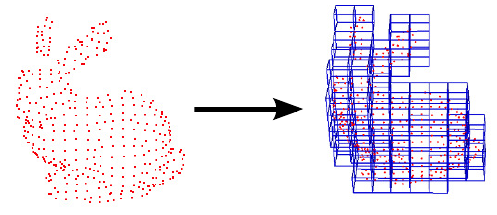
\includegraphics[width=0.8\linewidth]{figures/WorldModel/stanford_bunny.png}
\end{center}
   \caption[Example of Voxelization]{Illustration of Voxelization. On the left we have a point cloud of the ``Stanford Bunny''. This cloud is inserted into the voxel grid shown on the right, where all points falling within on grid unit, or voxel, are combined. From \url{http://www.pointclouds.org/} }
\label{fig:stanford_bunny}
\end{figure}
%------------------------------------------------------------------------

\begin{figure}[!t]
\begin{center}
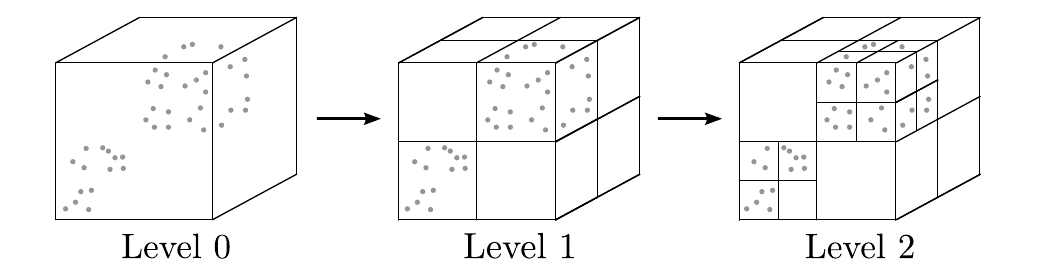
\includegraphics[width=\linewidth]{figures/WorldModel/voxel_grid_octree.png}
\end{center}
   \caption[Octree Voxelization]{Use of an octree for voxelization. The points are grouped into voxels by recursively subdividing the bounding box into its eight constituent octants. This recursion terminates when the box size has edge length equal to the voxel leaf size ${R}_{voxel}$.}
\label{fig:stanford_bunny}
\end{figure}

\begin{figure}[!t]
\begin{center}
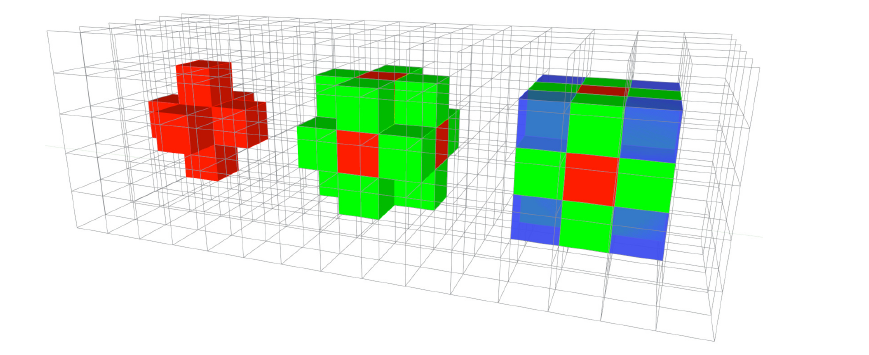
\includegraphics[width=0.9\linewidth]{figures/WorldModel/3d_nearest_neigh.png}
\end{center}
   \caption[Adjacency in a 3d Grid]{Adjacency in a 3d voxel grid. The 6-, 18-, and 26-neighborhoods share a face, edge, and vertex, respectively.}
\label{fig:3d_adjacency}
\end{figure}

\subsection{Octree Adjacency Graph}
\label{subsec:Adjacency}
In order to increase computational efficiency, we have developed an adjacency octree which maintains neighbor information within the octree leaves (i.e., the voxels). Adjacency is a key element of many methods, especially region growing algorithms, as it ensures that labels do not cross object boundaries which are disconnected in space. There are three definitions of adjacency in a voxelized 3D space; 6-,18-, or 26-adjacent. These share a face, faces or edges, and faces, edges, or vertices, respectively. In this work we use 26-adjacency exclusively, as the other lesser adjacencies might miss connections when surfaces are placed in certain configurations relative to the camera plane.

Throughout the rest of this work, we shall deal exclusively with voxels, rather than points, and shall always use our adjacency octree. As voxelization is a necessary pre-processing step for all of the algorithms we shall subsequently discuss, it can be assumed that adjacency information is always available in constant time. This is especially important for the clustering algorithm we introduce next.

\section{Geometrically Constrained Supervoxels}
\label{sec:Supervoxels}
In this Section we present  \acrfull{vccs}, a new method for generating superpixels and supervoxels from 3D point cloud data. The supervoxels produced by \gls{vccs} adhere to object boundaries better than state-of-the-art methods while remaining efficient enough to use in online applications. VCCS uses a variant of k-means clustering for generating its labeling of points, with two important constraints:

1. The seeding of supervoxel clusters is done by partitioning 3D space, rather than the projected image plane. This ensures that supervoxels are evenly distributed according to the geometry of the scene.

2. The iterative clustering algorithm enforces strict spatial connectivity of occupied voxels when considering points for clusters. This means that supervoxels strictly cannot flow across boundaries which are disjoint in 3D space, even though they are connected in the projected plane.
 
First, in \ref{subsec:Seeding} we shall describe how supervoxel seeds are generated and filtered, in \ref{subsec:Features} the features and distance measure used for clustering, and finally in \ref{subsec:FlowClustering} how the iterative clustering algorithm enforces spatial connectivity. Unless otherwise noted, all processing is being performed in the 3D voxelized space constructed from one or more RGB+D cameras (or any other source of point-cloud data). Furthermore, because we work exclusively in a voxel-cloud space (rather than the continuous point-cloud space), we shall adopt the following notation to refer to voxel at index $i$ within voxel-cloud $V$ of voxel resolution $r$:
\begin{equation} \label{eqn:Voxel}
{V}_{r}(i) = \mathbf{F}_{1..n}, 
\end{equation}
where $\mathbf{F}$ specifies a feature vector which contains $n$ point features (e.g. color, location, normals). 

\subsection{Spatial Cluster Seeding}
\label{subsec:Seeding}
The algorithm begins by selecting a number of seed points which will be used to initialize the supervoxels. In order to do this, we first divide the space into a voxelized grid with a chosen resolution ${R}_{seed}$, which is significantly higher than ${R}_{voxel}$. The effect of increasing the seed resolution ${R}_{seed}$ can be seen in Figure~\ref{fig:SegmentedDiffSeeds}. Initial candidates for seeding are chosen by selecting the voxel in the cloud nearest to the center of each occupied seeding voxel.    

Once we have candidates for seeding, we must filter out seeds caused by noise in the depth image. This means that we must remove seeds which are points isolated in space (which are likely due to noise), while leaving those which exist on surfaces. To do this, we establish a small search radius ${R}_{search}$ around each seed, and delete seeds which do not have at least as many voxels as would be occupied by a planar surface intersecting with half of the search volume (this is shown by the green plane in Figure~\ref{fig:SeedingDiagram}). Once filtered, we shift the remaining seeds to the connected voxel within the search volume which has the smallest gradient in the search volume. Gradient is computed as
\begin{equation} \label{eqn:Gradient}
\mathit{G}(i) = \sum_{k\in{V}_{adj}}{\frac{\parallel{V(i)-V(k)}\parallel{}_{CIELab}}{{N}_{adj}}};
\end{equation}
we use sum of distances in CIELAB space from neighboring voxels, requiring us to normalize the gradient measure by number of connected adjacent voxels ${N}_{adj}$. Figure~\ref{fig:SeedingDiagram} gives an overview of the different distances and parameters involved in seeding.

%------------------------------------------------------------------------
\begin{figure}
\begin{center}
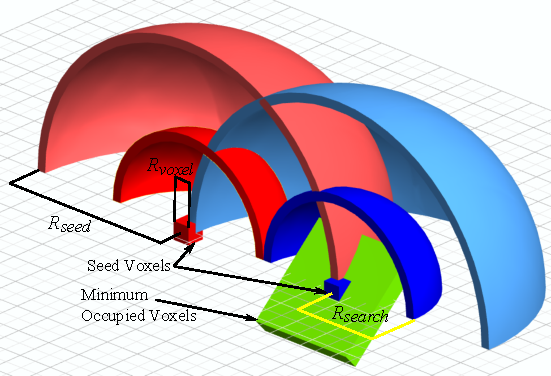
\includegraphics[width=0.9\linewidth]{figures/CVPR2013/MinimumOccupied.pdf}
\end{center}
   \caption[Seeding Parameters]{Seeding parameters and filtering criteria. ${R}_{seed}$ determines the distance between supervoxels, while ${R}_{voxel}$ determines the resolution to which the cloud is quantized. ${R}_{search}$ is used to determine if there are a sufficient number of occupied voxels to necessitate a seed. }
\label{fig:SeedingDiagram}
\end{figure}
%------------------------------------------------------------------------
%------------------------------------------------------------------------
\begin{figure}
\begin{center}
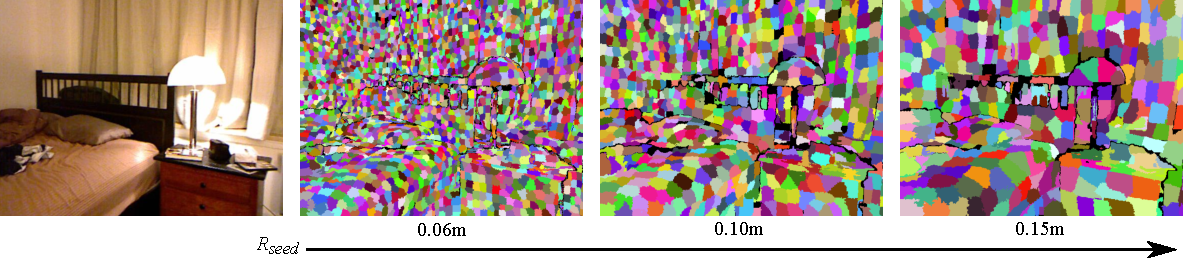
\includegraphics[width=1.0\linewidth]{figures/CVPR2013/IncreasingSeedSize.pdf}
\end{center}
   \caption[Seeding Size]{Image segmented using \gls{vccs} with seed resolutions of 0.1, 0.15 and 0.2 meters.}
\label{fig:SegmentedDiffSeeds}
\end{figure}
%------------------------------------------------------------------------
Once the seed voxels have been selected, we initialize the supervoxel feature vector by finding the center (in feature space) of the seed voxel and connected neighbors within 2 voxels. 

\subsection{Cluster Features and Distance}
\label{subsec:Features}
\gls{vccs} supervoxels are clusters in a 39 dimensional space, given as 
\begin{equation}
\label{eqn:FeatureSpace}
\mathbf{F} = [x,y,z,L,a,b,\textrm{FPFH}_{1..33}],
\end{equation}
where $x,y,z$ are spatial coordinates, $L,a,b$ are color in CIELab space, and $\textrm{FPFH}_{1..33}$ are the 33 elements of Fast Point Feature Histograms (FPFH), a local geometrical feature proposed by Rusu et al.\@ \cite{RusuFPFH}. FPFH are pose-invariant features which describe the local surface model properties of points using combinations of their \textit{k} nearest neighbors. They are an extension of the older Point Feature Histograms optimized for speed, and have a computational complexity of $O(n \cdot k)$.  

In order to calculate distances in this space, we must first normalize the spatial component, as distances, and thus their relative importance, will vary depending on the seed resolution ${R}_{seed}$. Similar to the work of Achanta et al.\@, \cite{SLICCompared} we have limited the search space for each cluster so that it ends at the neighboring cluster centers. This means that we can normalize our spatial distance $D_s$ using the maximally distant point considered for clustering, which will lie at a distance of $\sqrt{3} {R}_{seed}$. Color distance $D_c$, is the euclidean distance in CIELab space, normalized by a constant $m$. Distance in FPFH space, $D_f$, is calculated using the Histogram Intersection Kernel \cite{HistogramIntersection}. This leads us to a equation for normalized distance $D$:
\begin{equation}
\label{eqn:Distance}
D = \sqrt{\frac{\lambda D_c^2}{m^2}+\frac{\mu D_s^2}{3 {R}_{seed}^{2}}+\epsilon {D}_{HiK}^{2}},
\end{equation}
where $\lambda,\mu,$ and $\epsilon$ control the influence of color, spatial distance, and geometric similarity, respectively, in the clustering. In practice we keep the spatial distance constant relative to the other two so that supervoxels occupy a relatively spherical space, but this is not strictly necessary. For the experiments in this paper we have color weighted equally with geometric similarity.

\subsection{Flow Constrained Region Growing}
\label{subsec:FlowClustering}
Assigning voxels to supervoxels is done iteratively, using a local k-means clustering related to \cite{SLICCompared,DASP}, with the significant difference that we consider connectivity and flow when assigning pixels to a cluster. The general process is as follows: beginning at the voxel nearest the cluster center, we flow outward to adjacent voxels and compute the distance from each of these to the supervoxel center using Equation \ref{eqn:Distance}. If the distance is the smallest this voxel has seen, its label is set, and using the adjacency graph, we add its neighbors which are further from the center to our search queue for this label. We then proceed to the next supervoxel, so that each level outwards from the center is considered at the same time for all supervoxels. We proceed iteratively outwards until we have reached the edge of the search volume for each supervoxel (or have no more neighbors to check).

%------------------------------------------------------------------------
\begin{figure}[!t]
\begin{center}
   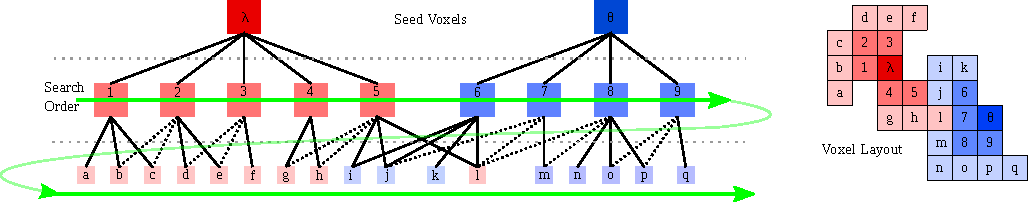
\includegraphics[width=0.95\linewidth]{figures/CVPR2013/SearchOrder.pdf}
\end{center}
   \caption[Voxel Search Order]{Search order for the flow constrained clustering algorithm (shown in 2D for clarity). Dotted edges in the adjacency graph are not searched, as the nodes have already been added to the search queue.}
\label{fig:ClusterSearch}
\end{figure}
%------------------------------------------------------------------------

This amounts to a breadth-first search of the adjacency graph, where we check the same level for all supervoxels before we proceed down the graphs in depth. Importantly, we avoid edges to adjacent voxels which we have already checked this iteration. The search concludes for a supervoxel when we have reached all the leaf nodes of its adjacency graph or none of the nodes searched in the current level were set to its label. This search procedure, illustrated in Figure~\ref{fig:ClusterSearch}, has two important advantages over existing methods:

1. Supervoxel labels cannot cross over object boundaries that are not actually touching in 3D space, since we only consider adjacent voxels, and 

2. Supervoxel labels will tend to be continuous in 3D space, since labels flow outward from the center of each supervoxel, expanding in space at the same rate.

Once the search of all supervoxel adjacency graphs has concluded, we update the centers of each supervoxel cluster by taking the mean of all its constituents. This is done iteratively; either until the cluster centers stabilize, or for a fixed number of iterations. For this work we found that the supervoxels were stable within a few iterations, and so have simply used five iterations for all presented results. 

\section{Sequential Update of Perceptual Model}
As an additional consideration, we have developed a scheme for adding new point clouds sequentially (as from a video stream) into an existing supervoxel octree. This is accomplished through a process which classifies voxels in the tree based on their behavior. As a first step, we insert points from the new point cloud into the octree, and initialize new leaves for voxels which did not exist previously. This results in an octree where leaves fall into three possible categories (illustrated in Figure~\ref{fig:VoxelVisibility}; they are either new, observed, or unobserved in the most recent observation. Handling of new leaves is straightforward; we simply calculate adjacency relations to existing leaves and flag them as unlabeled. 
\begin{figure}
  \centering
  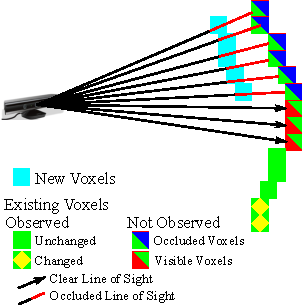
\includegraphics[scale=1.5]{figures/IROS2013/VoxelVisibility.pdf}
  \caption[Voxel Visibility]{Categorization of voxels based on new frame of data. Voxels fall into three categories, they are either new, observed or not observed in the frame. Furthermore, observed voxels can either have changed or remained the same, while voxels not observed in the frame are either occluded or no longer exist (in which case they should be deleted).}
  \label{fig:VoxelVisibility}
\end{figure}

To determine whether a leaf which existed previously has changed, we test the distance between the centroid of the points falling within its voxel (from the new frame) and its previous centroid. This is done in the same feature space used for growing the supervoxels, that is, we test whether the normal, color, and spatial location have varied more than a threshold value. This threshold is set to a relatively low constant value so that it favors false-positives (finding change when there was none), as they do not impact the tracking performance of the algorithm, but only have a slight effect on its run-time.  If a leaf is found to have changed, we remove its previous labeling. We also perform a global check to see if more than half of a supervoxels support has changed; if so, we completely remove the supervoxels label from all of its constituent voxels. 

Finally, we must consider how to handle leaves which were not observed in the inserted point cloud. Rather than simply prune them, we first check if it was possible to observe them from the viewpoint of the sensor which generated the input cloud. This occlusion check can be accomplished efficiently using the octree by determining if any voxels exist between unobserved leaves and the sensor viewpoint. If a clear line of sight exists from the leaf to the camera, it can safely be deleted. Conversely, if the path is obstructed, we "freeze" the leaf, meaning that it will remain constant until it is either observed or passes the line of sight test in a future frame (in which case, it can be safely deleted). This occlusion testing means that tracking of occluded objects is trivial, as occluded voxels remain in the observations which are used for tracking. This procedure results in what we term ``voxel-permanence'', as it results in voxels persisting through occlusions as seen in Figure \ref{fig:SequentialResults}. 

%------------------------------------------------------------------------
\begin{figure}[!t]
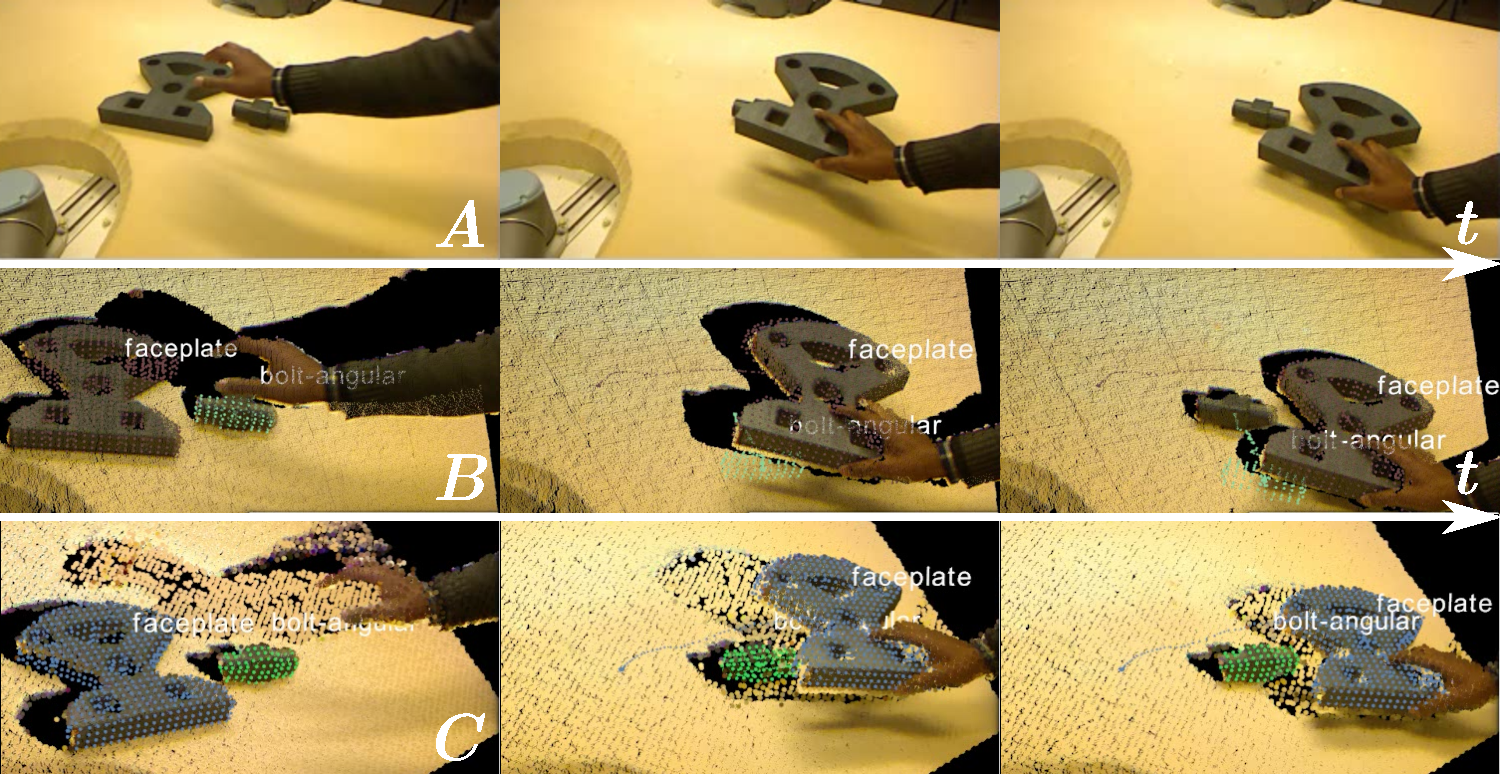
\includegraphics[width=\linewidth]{figures/WorldModel/sequential.pdf}
   \caption[Voxel Permanence]{Example of successful tracking of an object through complete occlusion using the sequentially updated world model and the concept of voxel permanence. Row A shows the original image frames - the bolt becomes occluded by the faceplate and cannot be seen by the sensor. Row B shows tracking failure using the raw 3D data - black ``holes'' behind the arm and faceplate are due to occlusion. Row C shows our model and tracked output - ``holes'' are now mostly filled in allowing tracking to succeed.}
\label{fig:SequentialResults}
\end{figure}
%------------------------------------------------------------------------

Once the octree voxels have been updated, we then proceed to update the supervoxels as before. That is, first we generate new seeds in regions of large unlabeled voxels, and then conduct the iterative region growing. This results in new supervoxels in regions which are new or changing, while leaving supervoxels in static and occluded regions unchanged. This reduces the tracking and segmentation problem to finding the best joint association of these new supervoxels with those from the prior time-step.

\section{Depth Dependent Voxel Grid}
So far we have described the main algorithm for generating supervoxels. Next we will introduce a depth transform which improves supervoxels by addressing the shortcomings of the adjacency octree upon which \gls{vccs} depends. As with any system which uses projective geometry, observations from a single RGB-D camera have a significant drawback - the level of detail decreases with increasing distance from the camera. In our case, this manifests as decreasing point density. In addition, the levels of both quantization and noise grow quadratically with distance \cite{ICCV11smisek, Khoshelham2012}. The combined effect of quantization and change in point density with depth results in inevitable failure of adjacency computation. At a certain distance (dependent on the voxel size $R_{voxel}$), the sparsity of observed points results in ``holes'' in the octree, and a break-down of adjacency. This has obvious negative consequences for flow-constrained algorithms such as \gls{vccs} which rely on spatial connectivity for clustering. 

We compensate for the loss of point density and quantization with increasing depth $z$ by transforming the points into a skewed space using the transformation $T:(x,y,z)\rightarrow(x',y',z')$ with
      \begin{align}
    \begin{aligned}
    x'= x/z,~~~~y'= y/z,~~~~z' = \log(z)
    \end{aligned}
      \end{align}
The division of the $x$ and $y$ coordinates by $z$ reverses the perspective transformation, equalizing the point density in the $x$-$y$-plane. Transforming the $z$ coordinate helps to deal with the effects of depth quantization by compressing points as depth increases. It is easy to show that the transformation has the following property:
\begin{align}
  \frac{\partial x'}{\partial x} = \frac{\partial y'}{\partial y} = \frac{\partial z'}{\partial z}~=\frac{1}{z}
\end{align}
Because the derivatives are equal, the local coordinate frame is stretched equally along all axes by the transformations. The important thing about this property is, that small cubic voxels are still cubic after the transformation. This leaves the geometry of space basically untouched in the foreground (if the voxel size is chosen sufficiently small), while distant voxels are strongly transformed to fill the ``empty'' space, compensating for reduced point density.

Rather than transforming the clouds back and forth, we instead transform the bins of the octree itself, creating an octree where bin volume (and thus, voxel size) effectively increases with distance from the camera viewpoint. Doing this directly within the octree allows us to determine adjacency as before (neighboring bins), even though distance between neighboring voxels increases with distance from the camera. Figure~\ref{fig:quantization_transform} illustrates the advantageous effect of this transformation on segmentation.

\begin{figure}
  \centering
  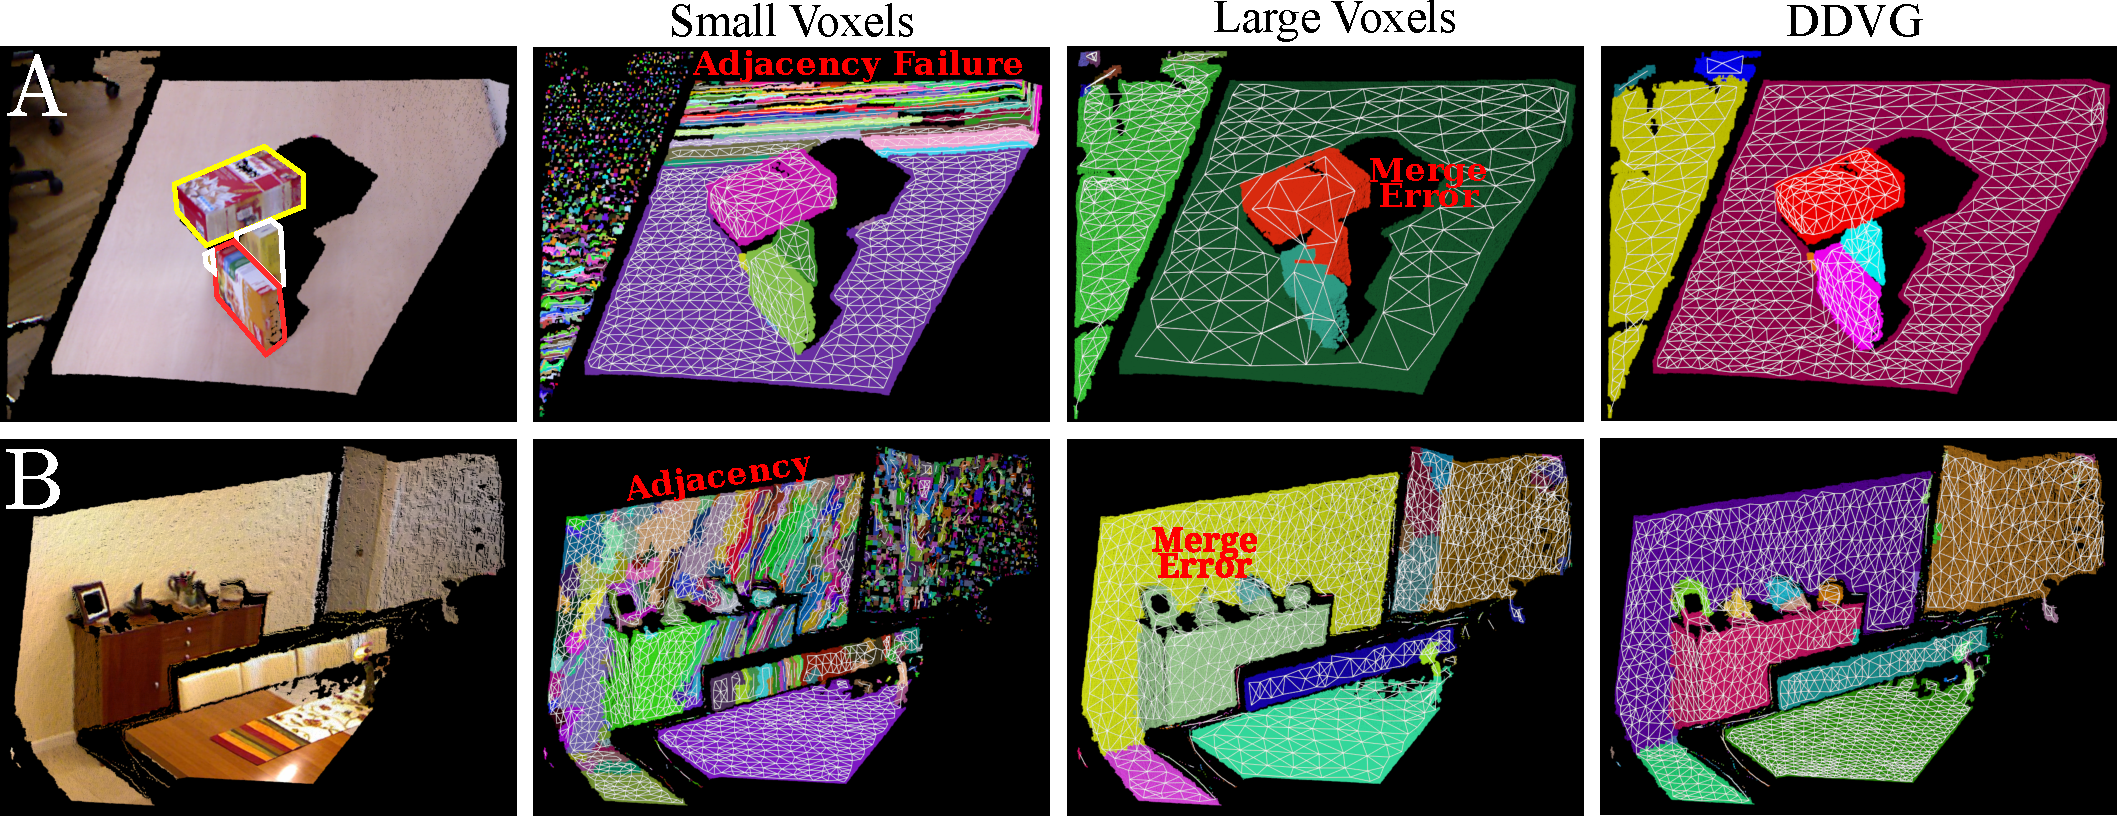
\includegraphics[width = \linewidth]{figures/CVPR2014/transform_results_v2}
\caption[Depth Adaptive Transform]{Two example point clouds \textbf{(A,B, left)} showing the need for the \gls{ddvg}. For better visibility outlines have been drawn around the boxes in A. Using \textit{Small Voxels} objects close to the camera can be segmented, but adjacency breaks down as the depth increases and the point density decreases. Using \textit{Large Voxels} corrects the adjacency graph in the background, but leads to objects being merged in the foreground due to the coarse resolution. Using \gls{ddvg}, the scale of the voxels gradually increases with distance from the camera -- adapting to the increased noise level and lower point density -- consequently adjacency is maintained and the segmentation of scenes with large depth variance is possible using fixed parameters. }
\label{fig:quantization_transform}
\end{figure}


\section{Locally Convex Connected Patches}
As an example of an application of supervoxels and the adjacency octree, we shall briefly present a segmentation method which breaks a supervoxel adjacency graph into meaningful segments by classifying whether an edge $e=(\vec p_i, \vec p_j)$ between two supervoxels is convex or concave. This classification is based on an \emph{\gls{ecc}}, which considers adjacent supervoxels with centroids at the positions $\vec x_1,\vec x_2$ and normals $\vec n_1, \vec n_2$. Whether the connection between these is convex or concave can be inferred from the relation of the surface normals to the vector joining their centroids - an overview of the this algorithm is given in Figure~\ref{fig:flow}.

\begin{figure}
\centering
  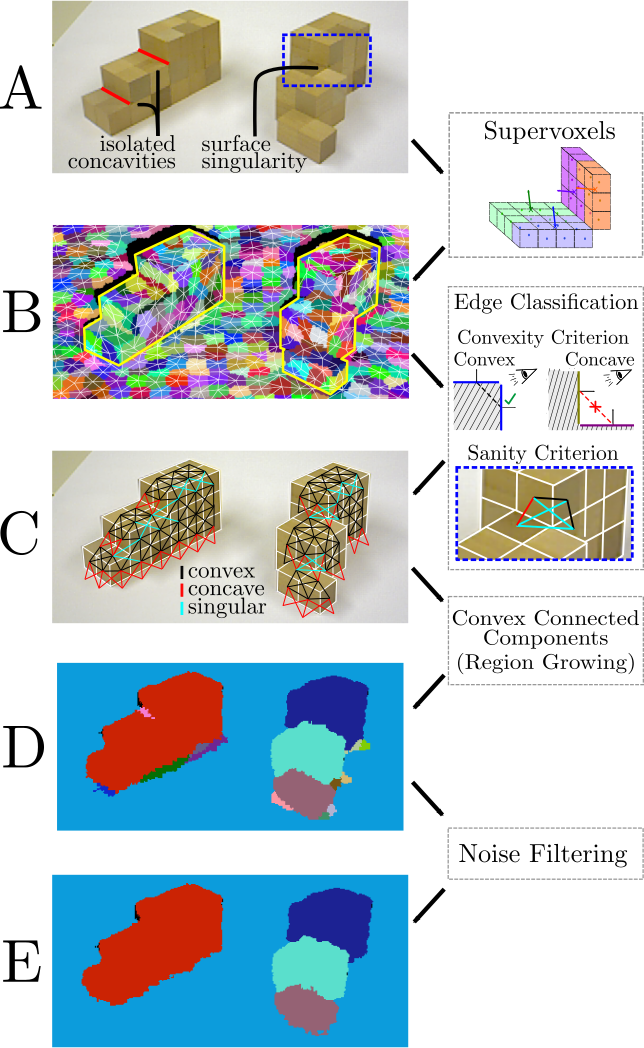
\includegraphics[width=0.8\linewidth]{figures/CVPR2014/flow_diagram}
    \caption[Flow Diagram of LCCP]{Flow diagram of the segmentation algorithm. \textbf{A)} RGB images corresponding to the point clouds of the scene. The red lines show two isolated concavities. The blue box shows an area with a surface singularity. \textbf{B)} Supervoxel adjacency graph. \textbf{C)} Model depicting the classified graph. Black lines denote convex connections, red lines concave ones and turquois lines singular connections (those, where two patches are connected only in a single point). \textbf{D)} Segmentation result; object labels are shown by different colors. \textbf{E)} Final result after noise filtering. The right column illustrates the supervoxel patches and the convexity and sanity criteria used for edge classification.}
  \label{fig:flow}
\end{figure}

The angle of the normals to the vector $\vec d = \vec x_1-\vec x_2$ joining the centroids can be calculated using the identity for the dot product $\vec a\cdot \vec b = |\vec a|\cdot |\vec b|\cdot \cos(\alpha)$ with $\alpha = \measuredangle(\vec a,\vec b)$. For \textit{convex} connections, $\alpha_1$ is smaller than $\alpha_2$. This can be expressed as:
  \begin{equation*}
    \alpha_1 < \alpha_2 \Rightarrow \cos(\alpha_1) - \cos(\alpha_2) > 0 \Leftrightarrow \vec {n_1}\cdot \hat d - \vec {n_2}\cdot \hat d > 0,
  \end{equation*}
where $\hat d = \frac{\vec{x_1}-\vec{x_2}}{||\vec{x_1}-\vec{x_2}||}$. Similarly, for a \textit{concave} connection we get:
  \begin{equation*}
    \alpha_1 > \alpha_2 \Leftrightarrow \vec {n_1}\cdot \hat d - \vec {n_2}\cdot \hat d < 0.
  \end{equation*}
Note that these operations are commutative, thus the choice of which patch is $\vec x_1$, does not change the result. Also the criterion is still valid if the $\vec x_i$ are displaced, as long as they stay within the surface.

To compensate for noise in the RGB-D data, a bias is introduced to treat concave connections with very similar normals, that is
\begin{align*}
  \beta = \measuredangle(\vec n_1,\vec n_2) = |\alpha_1-\alpha_2| = \cos^{-1}(\vec{n_1}\cdot \vec{n_2}) < \beta_\text{Thresh}~,
\end{align*}
as convex, since those usually represent flat surfaces. Depending on the value of the \textit{concavity tolerance threshold} $\beta_\text{Thresh}$, concave surfaces with low curvature are seen as convex and thus merged in the segmentation. This behavior may be desired to ignore small concavities. We set:
\begin{align}
  \text{CC}_b(\vec p_i, \vec p_j) :=
  \left\{\begin{array}{lc}
          \text{true} & \left(\vec {n_1} - \vec {n_2} \right) \cdot \hat d  > 0~ \lor~ (  \beta < \beta_\text{Thresh} )\\
            \text{false} & \text{otherwise.}\\
          \end{array} \right.
  \label{eqn:CC}
\end{align}

where the variable $CC_b$ defines the {\em basic convexity criterion}. However, local errors in the feature estimation caused by noise in the data can propagate very easily, potentially leading to errors in the resulting segmentation. This also makes the recognition of small concavities harder, as subtle features are more sensitive to noise. To improve on this we also include neighborhood information in the classification of edges: For a convex edge $e=(\vec p_i, \vec p_j)$, we require that there exists a common neighbor $\vec p_c$ of $\vec p_i$ and $\vec p_j$ that has a convex connection to both.

Thus we define \textit{extended convexity} $CC_e$:
\begin{align}
  \begin{aligned}
   \text{CC}_e (\vec p_i, \vec p_j) = \text{CC}_b(\vec p_i, \vec p_j) \land \text{CC}_b(\vec p_i, \vec p_c) \\ \land \text{CC}_b(\vec p_j, \vec p_c)
  \end{aligned}
\end{align}

With extended convexity, more evidence is necessary for a connection to be labeled as convex. 

As in \gls{vccs}, clusters are found in \gls{lccp} using a region growing process: First, an arbitrary seed supervoxel is chosen and labeled. This label is then propagated over the graph with a depth search that is only allowed to grow over convex edges. Once no new supervoxel can be assigned to the segment, we choose a new seed supervoxel that has not been labeled and propagate the new label as before, repeating the process until all supervoxels have been labeled. Note that all of the criteria in \gls{lccp} are commutative, so the output of the region growing does not depend on the choice of the seeds.

\section{Experimental Results}
\subsection{Datasets}
In the following sections we present quantitative results for \gls{vccs} and \gls{lccp}. We compare both to state-of-the-art methods on the \textit{NYU Indoor Dataset}\cite{Silberman:ECCV12} and \textit{Object Segmentation Database}\cite{Richtsfeld:IROS12}. Before giving results, we shall first describe the datasets as well as the procedure for scoring results using 2D ground-truth.

\subsubsection{Object Segmentation Database (OSD)}
The \textit{Object Segmentation Database} (OSD-v0.2) was proposed by Richtsfeld \textit{et al.}\cite{Richtsfeld:IROS12} in 2012. It consists of 111 cluttered scenes of objects on a table, taken with close proximity to the pictured objects. The scenes contain multiple objects, which have mostly box-like or cylindrical shape, with partial and full occlusions and heavy clutter in 2D as well as 3D. Importantly, most objects in the data set are \textit{simple}, that is, consist of only a single part. This makes the ground-truth data relatively non-ambiguous.

\begin{figure}
 \centering
 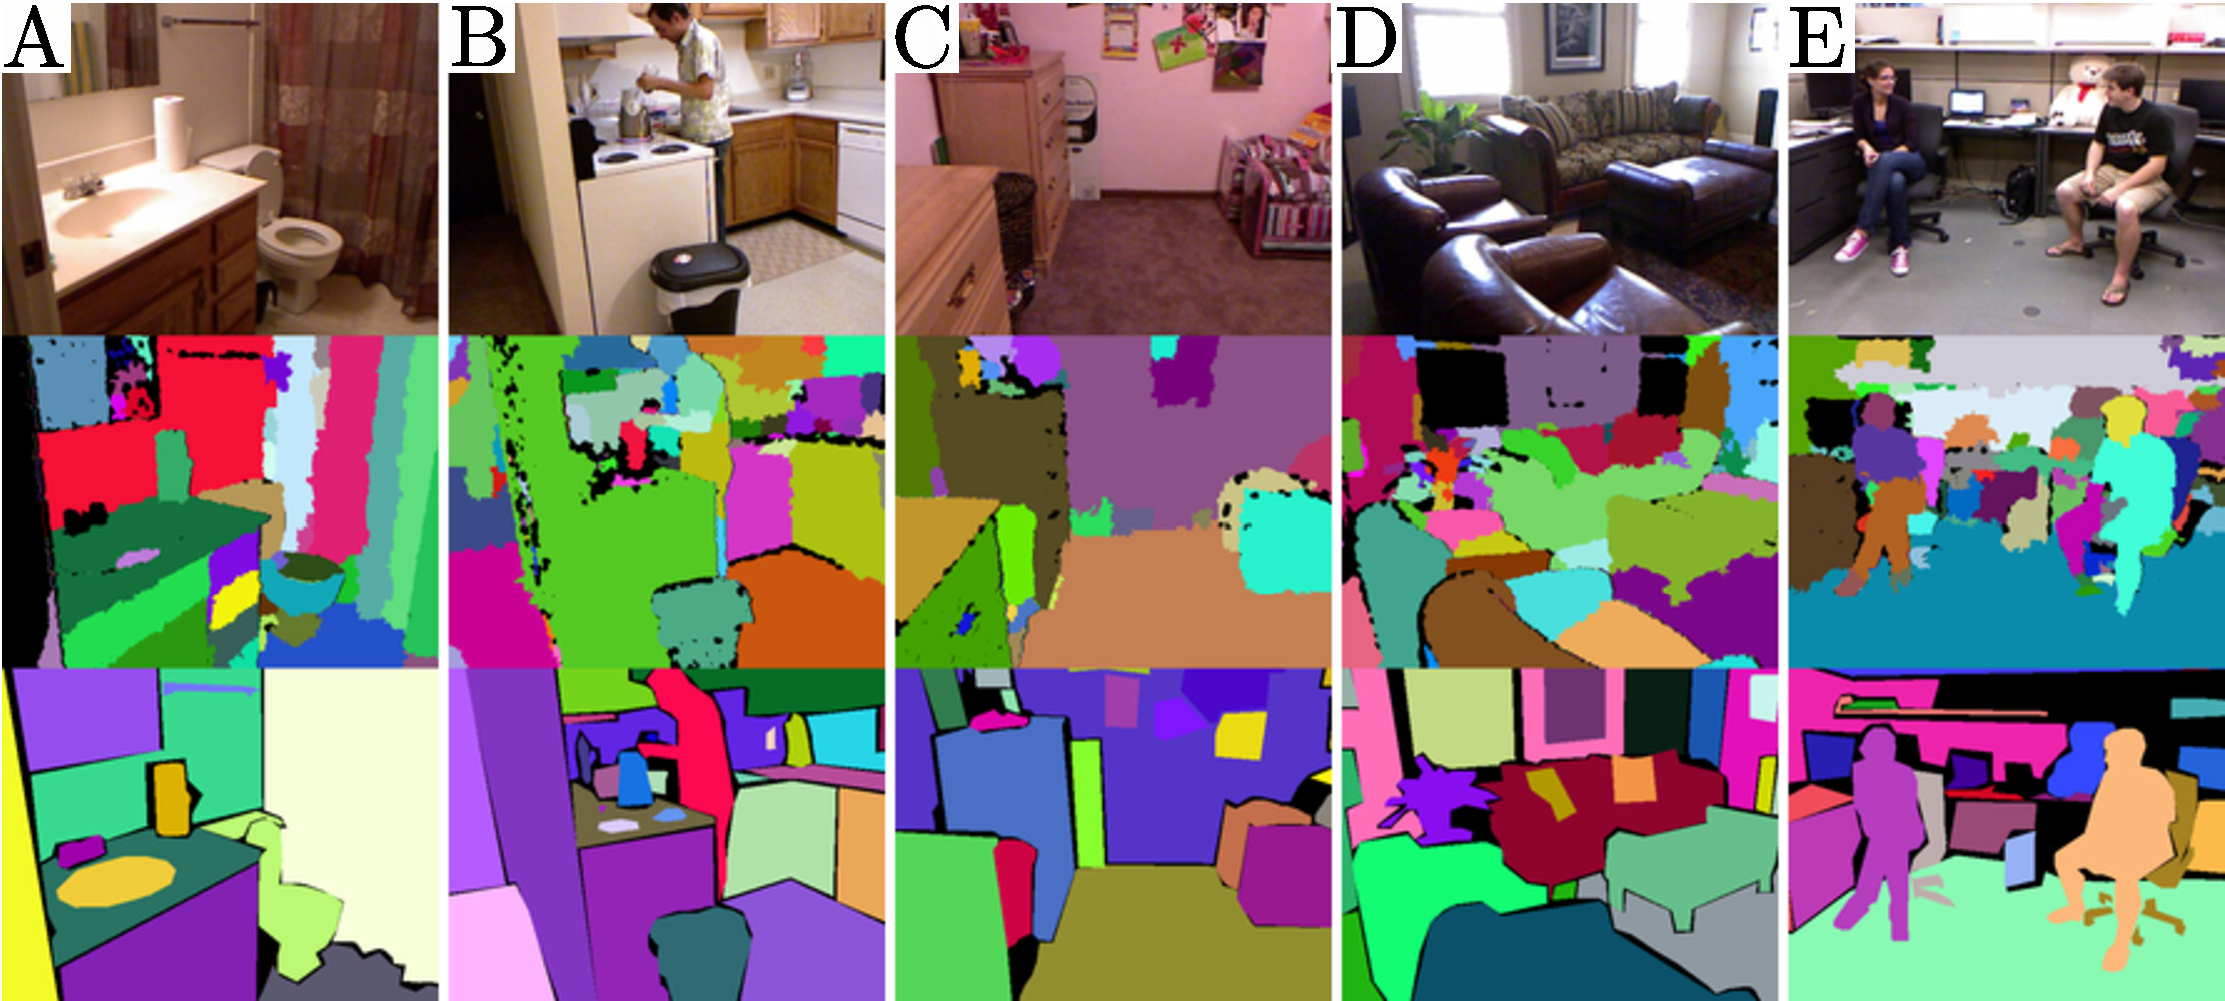
\includegraphics[width=1\linewidth]{figures/CVPR2014/nyu_examples.pdf}
 \caption[NYU Dataset Examples]{Example results for scenes from the NYU dataset using unsmoothed depth. Black areas indicate missing depth. Top row: rgb images. Mid. row: segmentation result. Bottom row: ground truth. Parameters A-C: $R_{voxel}=0.0075$, $R_{seed}=0.03$ and $\beta_\text{Thresh}=8^\circ$. Parameters D-E: $R_{voxel}=0.01$, $R_{seed}=0.04$ and $\beta_\text{Thresh}=10^\circ$ (identical to quantitative results, see Tab. \ref{tab:res_lccp_nyu}).}
 \label{fig:nyu_examples}
\end{figure}

\subsubsection{NYU Indoor Dataset (NYU)}
The \textit{NYU Indoor Dataset}\footnote{\url{http://cs.nyu.edu/~silberman/datasets/nyu_depth_v2.html}} (NYUv2) from Silberman \textit{et al.}\cite{Silberman:ECCV12} is a large and complex dataset, consisting of 1449 cluttered indoor scenes. The data consists of pairs of aligned RGB and depth images, along with human annotated densely labeled ground truth. The images were captured in diverse indoor scenes, and present many difficulties for segmentation algorithms such as varied illumination and many small similarly colored objects. Examples of typical scenes are shown in Figure~\ref{fig:ExampleSegmentations}. One main difficulty presented by the dataset is that the distance to objects from the camera is quite large in the dataset. This results in significant depth quantization artifacts as well as few data points for many objects. Additionally, depth is often missing for extensive portions of many of the images, due to limitations of the Kinect sensor (e.g. reflective, transparent surfaces - windows are especially problematic). Silberman \textit{et al.} attempt to correct for these errors using a hole filling algorithm (smoothdepth), which estimates depth for missing areas based on the scheme from Levin \textit{et al.}\cite{Levin2004}.

%------------------------------------------------------------------------
\begin{figure}
\begin{center}
%\fbox{\rule{0pt}{2.4in} \rule{0.9\linewidth}{0pt}}
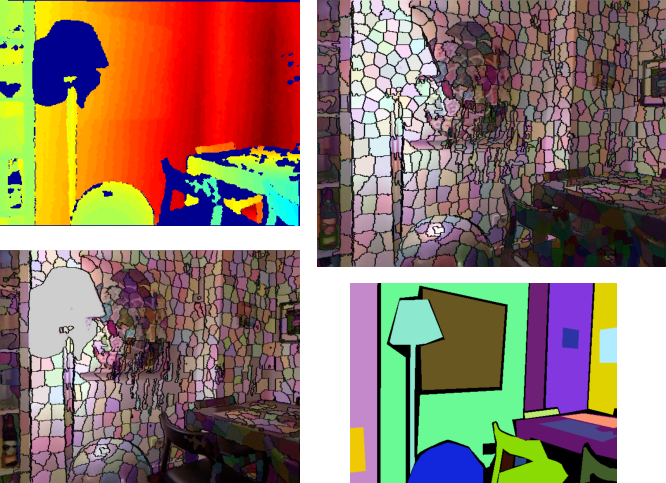
\includegraphics[width=0.9\linewidth]{figures/CVPR2013/BackTo2D.pdf}
\end{center}
   \caption[2D Hole Filling]{Example of hole-filling for images after returning from voxel-cloud to the projected image plane. Depth data, shown in the top left, has holes in it, shown as dark blue areas (here, due to the lamp interfering with the Kinect). The resulting supervoxels do not cover these holes as shown in the bottom left, since the cloud has no points in them. To generate a complete 2D segmentation, we fill these holes in using the SLIC algorithm, resulting in a complete segmentation, seen in the top right. The bottom right shows human annotated ground truth for the scene. }
\label{fig:ReturnToPlane}
\end{figure}
%------------------------------------------------------------------------

%------------------------------------------------------------------------
%\begin{figure}
%\begin{center}
%\includegraphics[width=1.01\linewidth]{figures/CVPR2013/Multiview.pdf}
%\end{center}
%   \caption[Supervoxels from Multiple Views]{Over-segmentation of a cloud from the RGB-D scenes dataset\cite{RGBDDataset}. The cloud is created by aligning 180 Kinect frames, examples of which are seen on the left side. The resulting cloud has over 3 million points, which reduces to 450k points at ${R}_{voxel}=0.01m$ and 100k points with ${R}_{voxel}=0.02m$. Over-segmentation of these take 6 and 1.5 seconds, respectively (including voxelization).}
%\label{fig:MultiViewCloud}
%\end{figure}
%------------------------------------------------------------------------

%------------------------------------------------------------------------
\begin{figure}
\begin{center}
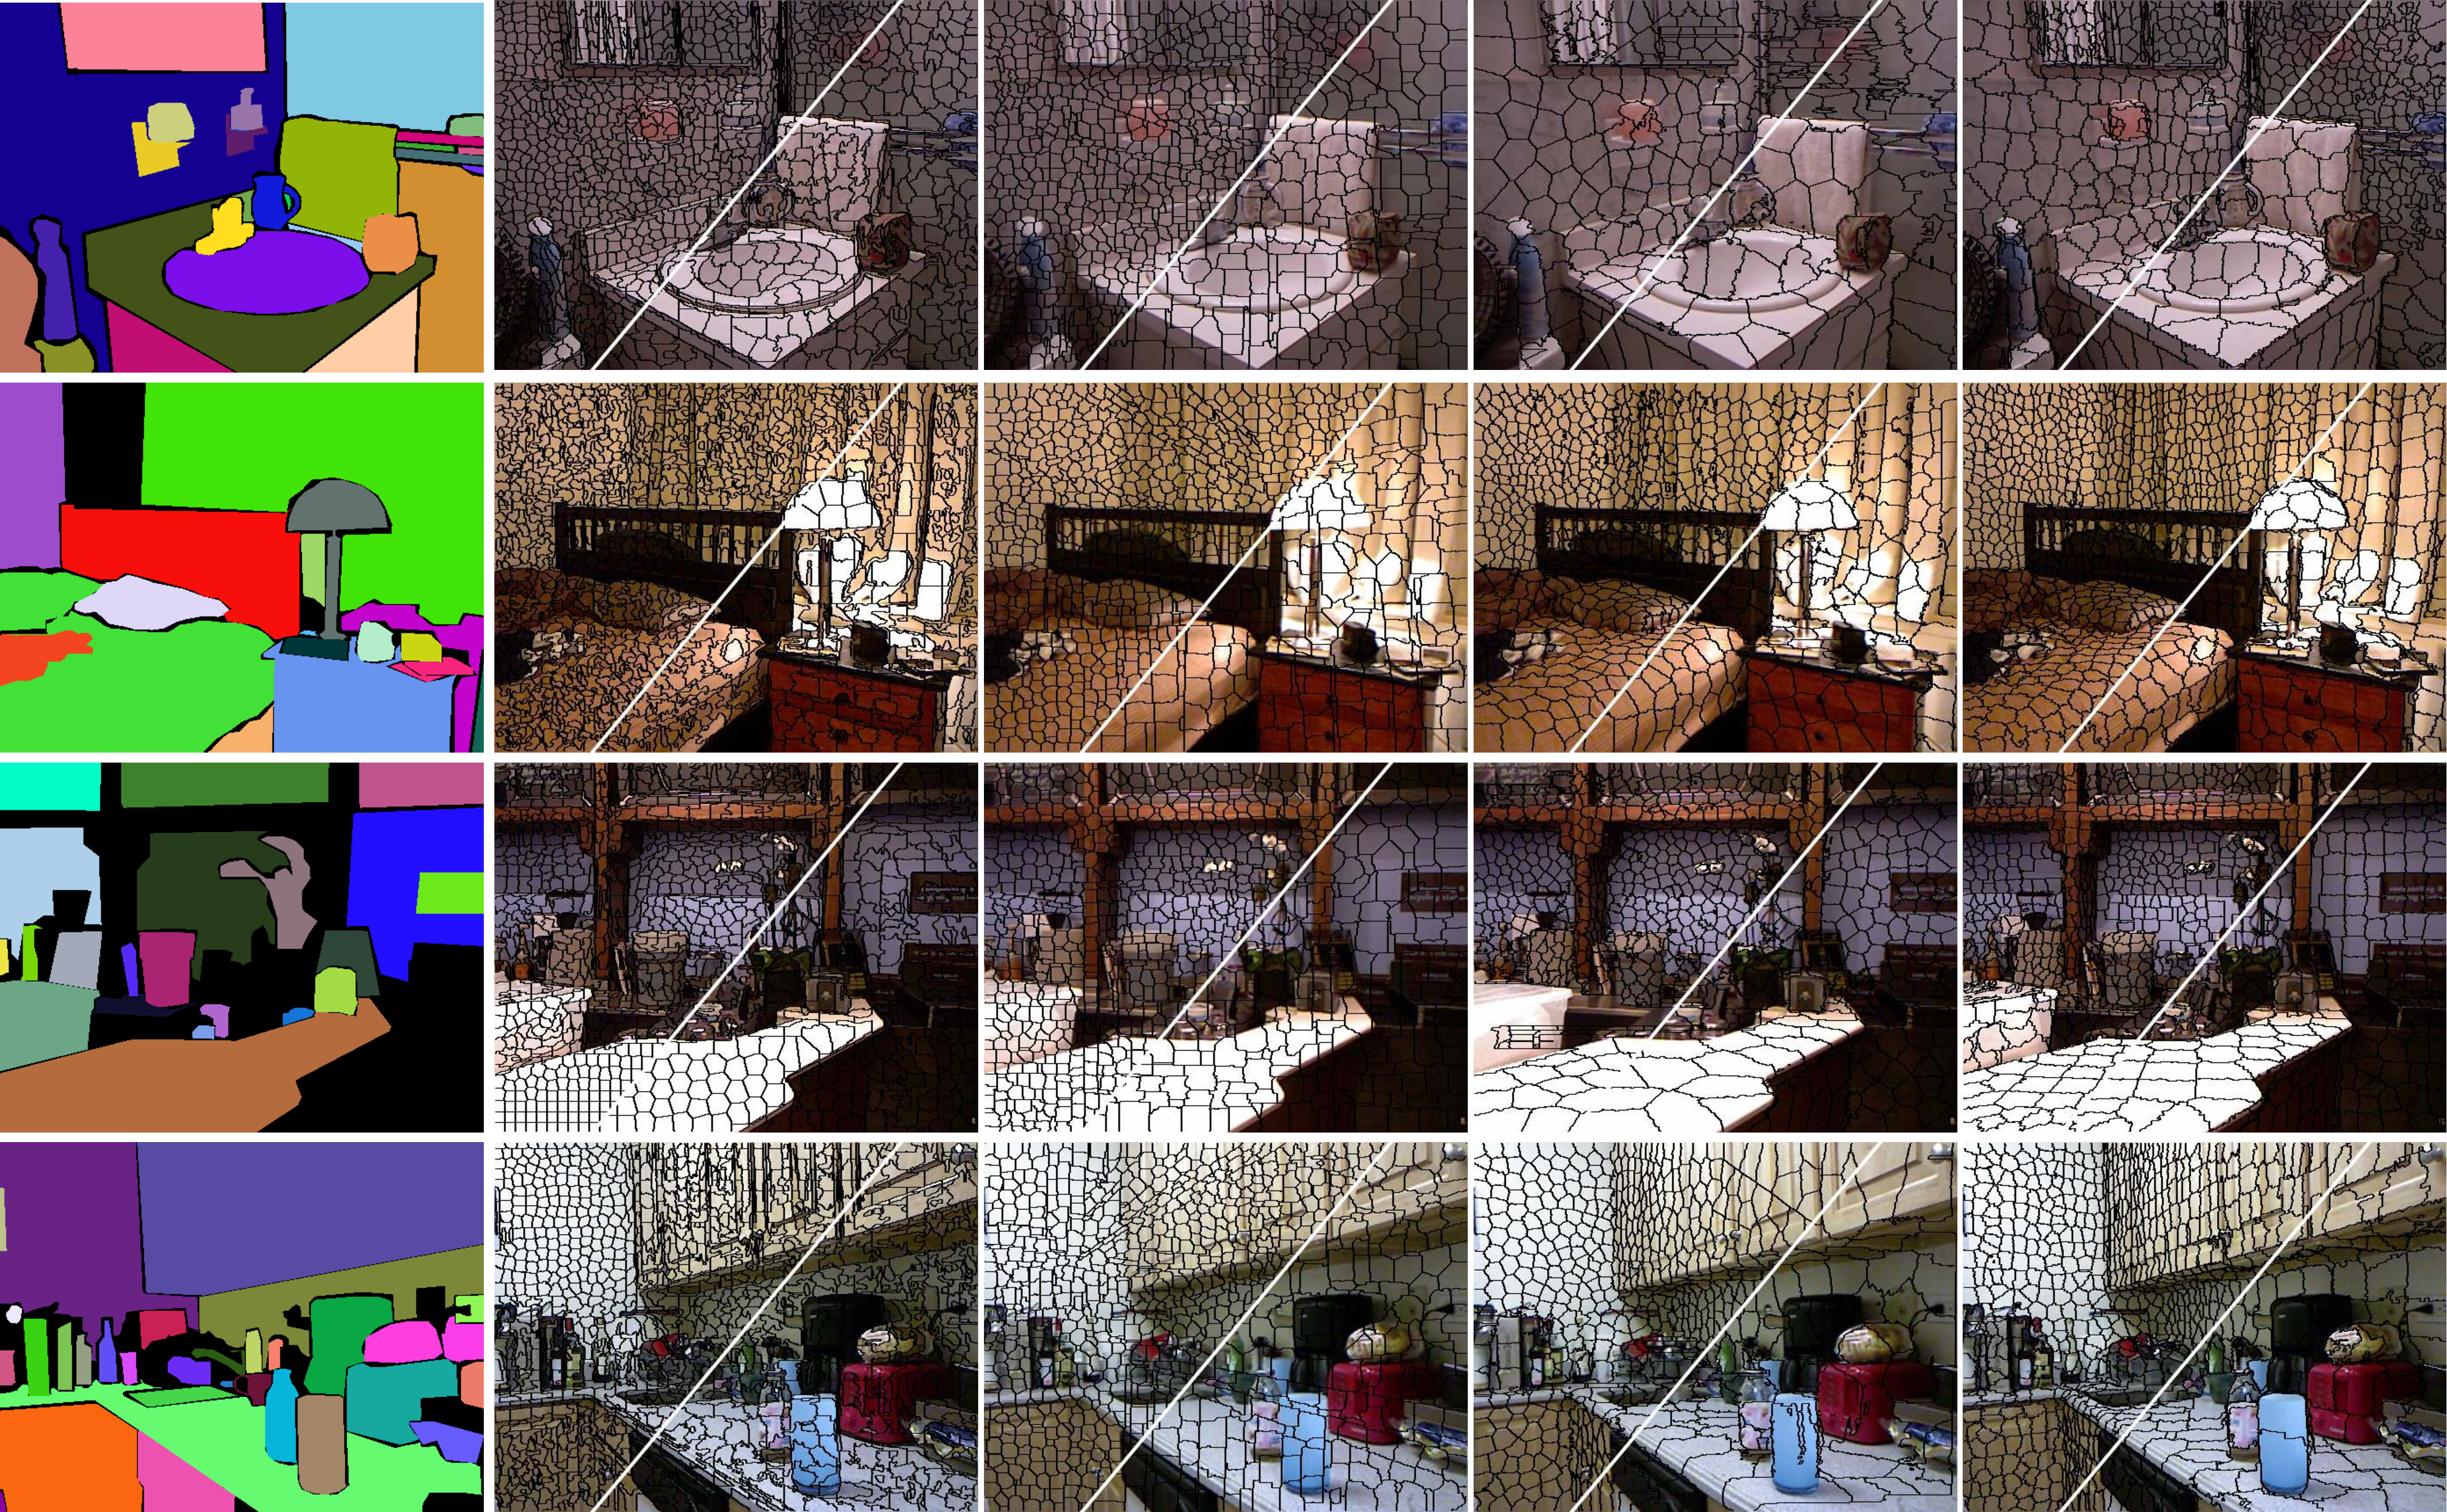
\includegraphics[width=1.01\linewidth]{figures/CVPR2013/Comparison_Segmentation_Small.pdf}
\end{center}
   \caption[Superpixel Comparison]{Examples of under-segmentation output. From left to right- ground truth annotation, SLIC, GCb10, DASP, and \gls{vccs}. Each is shown with two different superpixel densities.}
\label{fig:ExampleSegmentations}
\end{figure}
%------------------------------------------------------------------------

\subsubsection{Returning to the Projected Plane}
RGB+D sensors produce what is known as an organized point cloud- a cloud where every point corresponds to a pixel in the original RGB and depth images. When such a cloud is voxelized, it necessarily loses this correspondence, and becomes an unstructured cloud which no longer has any direct relationship back to the 2D projected plane. As such, in order to compare results with existing 2D methods we were forced to devise a scheme to apply supervoxel labels to the original image. 

To do this, we take every point in the original organized cloud and search for the nearest voxel in the voxelized representation. Unfortunately, since there are blank areas in the original depth image due to such factors as reflective surfaces, noise, and limited sensor range, this leaves us with some blank areas in the output labeled images. To overcome this, we fill in any large unlabeled areas using the SLIC algorithm. This is not a significant drawback, as the purpose of the algorithm is to form supervoxels in 3D space, not superpixels in the projected plane, and this hole-filling is only needed for comparison purposes. Additionally, the hole filling actually makes our results worse, since it does not consider depth, and therefore tends to bleed over some object boundaries that were correctly maintained in the supervoxel representation. An example of what the resulting segments look like before and after this procedure are shown in Figure~\ref{fig:ReturnToPlane}. 

\subsection {Supervoxels}
\label{sec:Evaluation}
In order to evaluate the quality of supervoxels generated by \gls{vccs}, we performed a quantitative comparison with three state-of-the-art superpixel methods using publicly available source code. 
We selected the two 2D techniques with the highest published performance from a recent review \cite{SLICCompared}: a graph based method, GCb10 \cite{SuperpixelsSupervoxels}\footnote{\url{http://www.csd.uwo.ca/~olga/Projects/superpixels.html}}, and a gradient ascent local clustering method, SLIC \cite{SLICCompared}\footnote{\url{http://ivrg.epfl.ch/supplementary_material/RK_SLICSuperpixels/index.html}}.
Additionally, we selected another method which uses depth images, DASP\cite{DASP}\footnote{\url{https://github.com/Danvil/dasp}}.
Examples of over-segmentations produced by the methods are given in Figure~\ref{fig:ExampleSegmentations}.
%------------------------------------------------------------------------
\begin{figure}
\begin{center}
%\includegraphics[width=0.8\linewidth,type=eps,ext=.eps,read=.eps]{Figures/boundary}
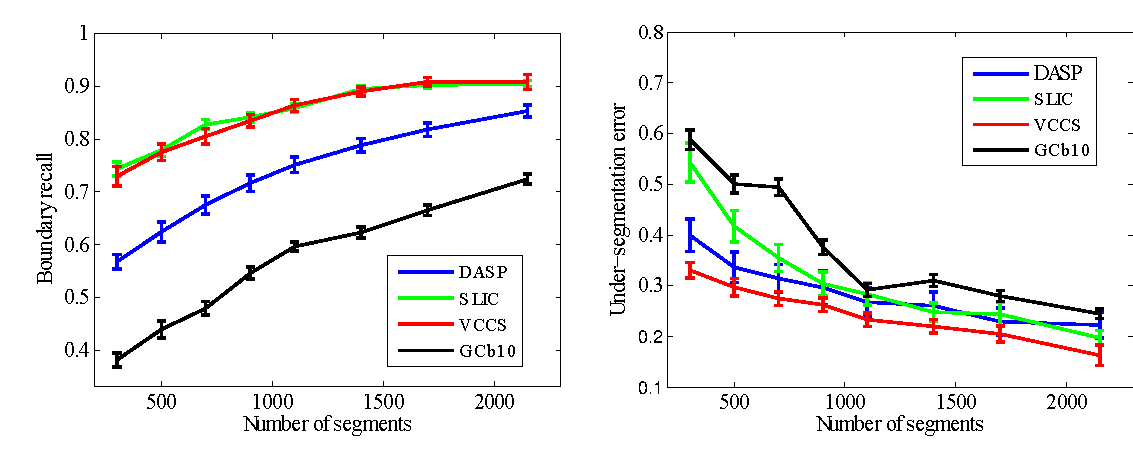
\includegraphics[width=0.95\linewidth]{figures/CVPR2013/Performance.pdf}
\end{center}
   \caption[Boundary Recall \& Undersegmentation Error]{Boundary recall and under-segmentation error for SLIC, GCb10, DASP, and \gls{vccs}.}
\label{fig:BoundaryRecall}
\label{fig:UndersegError}
\end{figure}
%------------------------------------------------------------------------
\subsubsection{Object Boundary Adherence}
The most important property for superpixels is the ability to adhere to, and not cross, object boundaries. To measure this quantitatively, we have used two standard metrics for boundary adherence- boundary recall and under-segmentation error\cite{Turbopixels, SuperpixelsSupervoxels}. Boundary recall measures what fraction of the ground truth edges fall within at least two pixels of a superpixel boundary. High boundary recall indicates that the superpixels properly follow the edges of objects in the ground truth labeling. The results for boundary recall are given in Figure~\ref{fig:BoundaryRecall}. As can be seen, \gls{vccs} and SLIC have the best boundary recall performance, giving similar results as the number of superpixels in the segmentation varies. 

Under-segmentation error measures the amount of leakage across object boundaries. For a ground truth segmentation with regions $g_1,...,g_M$, and the set of superpixels from an over-segmentation, $s_1,...s_K$, under-segmentation error is defined as 
\begin{equation}
\label{eqn:UndersegError}
{E}_{useg}=\frac{1}{N} \left[ \sum_{i=1}^{M}{\left(\sum_{s_j \mid s_j \cap g_i}{|s_j|}\right)-N} \right],
\end{equation}
where $s_j \mid s_j \cap g_i$ is the set of superpixels required to cover a ground truth label $g_i$, and $N$ is the number of labeled ground truth pixels. A lower value means that less superpixels violated ground truth borders by crossing over them. Figure~\ref{fig:UndersegError} compares the four algorithms, giving under-segmentation error for increasing superpixel counts. \gls{vccs} outperforms existing methods for all superpixel densities. 

\subsubsection{Time Performance}
As superpixels are used as a preprocessing step to reduce the complexity of segmentation, they should be computationally efficient so that they do not negatively impact overall performance. To quantify segmentation speed, we measured the time required for the methods on images of increasing size (for the 2D methods) and increasing number of voxels (for \gls{vccs}). All measurements were recorded on an Intel Core i7 3.2Ghz processor, and are shown in Figure~\ref{fig:SegmentationSpeed}. \gls{vccs} shows performance competitive with SLIC and DASP (the two fastest superpixel methods in the literature) for voxel clouds of sizes which are typical for Kinect data at ${R}_{voxel}=0.008m$ (20-40k voxels). It should be noted that only \gls{vccs} takes advantage of multi-threading (for octree, kd-tree, and FPFH computation), as there are no publicly available multi-threaded implementations of the other algorithms.  

%------------------------------------------------------------------------
\begin{figure}
\begin{center}
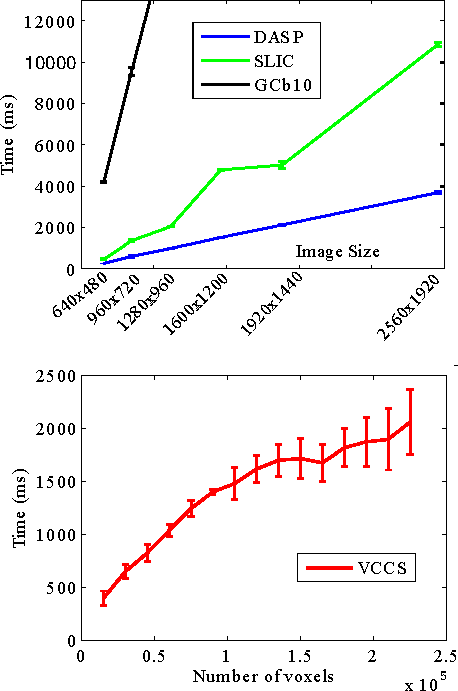
\includegraphics[width=0.95\linewidth]{figures/CVPR2013/Speed.pdf}
\end{center}
   \caption[Segmentation Speed]{Speed of segmentation for increasing image size and number of voxels. Use of GCb10 rapidly becomes unfeasible for larger image sizes, and so we do not adjust the axes to show its run-time. The variation seen in \gls{vccs} run-time is due to dependence on other factors, such as ${R}_{seed}$ and overall amount of connectivity in the adjacency graphs.}
\label{fig:SegmentationSpeed}
\end{figure}
%------------------------------------------------------------------------

\subsection{Locally Convex Connected Patches}

We compare segments found using \gls{lccp} against ground truth using three standard measures: \textit{Weighted Overlap} (WOv), which is a summary measure proposed by Silberman \textit{et al.} \cite{Silberman:ECCV12}, as well as \textit{false negative} ($fn$) and \textit{false positive} ($fp$) scores from \cite{Ritter2012} and \textit{over-} ($F_{os}$) and \textit{under-segmentation} ($F_{us}$) from \cite{Richtsfeld:IROS12}.

\begin{figure}
 \centering
 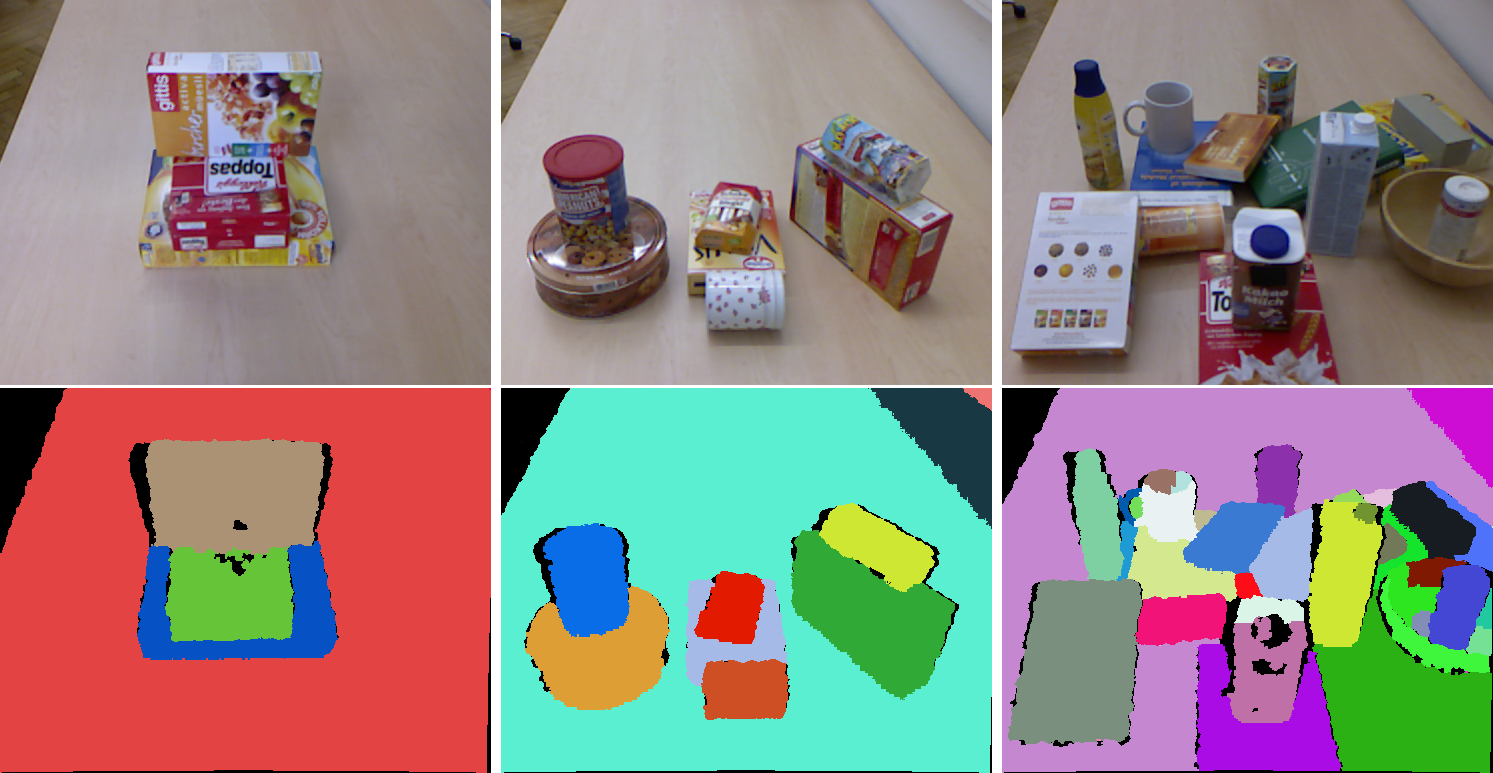
\includegraphics[width=1\linewidth]{figures/CVPR2014/osd_examples}
 \caption[OSD Dataset Examples]{ Example results for the OSD dataset. Points beyond a distance of 2m were cropped for visualization. Parameters: $R_{voxel}=0.005$, $R_{seed}=0.02$, $\beta_\text{Thresh}=10^\circ$.  }
 \label{fig:OSD_results}
\end{figure}

%%%%%%%%%%%%%%%%%%%%%%%%%%%%%%%%%%%%%%%%%%%%%%%%%%%%%%%%%%%%%%%%%%%%%%%%%%%%%%%%%%%%%%%%%%%%
 \begin{table*}[!ht]
   \small
   \centering
    \begin{tabular}{c||c||c||cc||cc||c||c}
    \multirow{2}{*}{Method} & Learned & WOv     & \multicolumn{2}{c||}{$fp$} & \multicolumn{2}{c||}{$fn$} & $F_{os}$ & $F_{us}$ \\ \cline{3-9}
    ~                       & Features & Mean   & Mean  & SD     & Mean  & SD    & Mean   & Mean   \\ \hline\hline
    LCCP            &  NO LEARNING & 88.7\% &  4.8\% & 2.6\%  & 8.3\% & 8.7\% & 7.4\%  & 4.7\%  \\ \hline
    Richtsfeld~\cite{Richtsfeld:IROS12}  & RGB-D,Texture,Geometry & -      & -          & -      & -     & -     & 4.5\%  & 7.9\%  \\ \hline
    {\"U}ckermann~\cite{Ritter2012} & NO LEARNING & -      & 1.9\% & 3.3\%  & 7.8\% & 7.3\% & -      & -      \\ \hline
    \end{tabular}
    \caption[Segmentation Results on OSD Dataset]{Comparison of different segmentation methods on the OSD dataset using weighted overlap \textit{WOv} (the higher, the better), false positives \textit{$f_p$}, false negatives \textit{$f_n$}, as well as over- and under-segmentation \textit{$F_{os}$} and \textit{$F_{us}$} (the lower, the better). LCCP results were produced with voxel resolution $R_{voxel} = 0.005$, seed resolution $R_{seed} = 0.02$ and concavity tolerance angle $\beta_\text{Tresh}=10^\circ$.}
    \label{tab:res_stat}
\end{table*}

The qualitative examples from the OSD dataset (Figure~\ref{fig:OSD_results}) show that \gls{lccp} performs very well in the segmentation of cluttered scenes. The object separation can be intuitively understood: all objects present in the scenes are separated by concave boundaries, i.e. a line connecting neighboring surfaces of two different objects always travels through ``air''. This is also true for the boundary between an object and the supporting surface. As a consequence, objects that have a convex shape are correctly captured as one segment and separated from the other objects. Hollow objects (bowls, cups etc.) can be observed to show multiple segments inside, because the orientation of surface normals changes strongly on these concave surfaces. The quantitative results (Table~\ref{tab:res_stat}) demonstrate that the approach is able to compete with state-of-the-art methods in the task of segmenting cluttered scenes with 'single-part' objects. 

\begin{table*}
  \centering
  \begin{tabular}{c|c|c|c}
%   \textbf{Overlap} & \textbf{Weighted Overlap} & \textbf{oversegmentation} & \textbf{undersegmentation} \\
  Method & Learned Features & Depth Data  & WOv\\ \hline \hline
  \multirow{2}{*}{LCCP} & NO LEARNING & depth & 53.6\% \\ \cline{2-4}
                                           & NO LEARNING & smoothdepth & 53.8\% \\ \hline
  LCCP + ext. convexity & NO LEARNING & smoothdepth &  57.6\% \\ \hline \hline
  \multirow{4}{*}{Silberman \textit{et al.}\cite{Silberman:ECCV12}} & RGB  & - &  50.3\% \\ \cline{2-4}
                                           & Depth & both  & 53.7\% \\ \cline{2-4}
                                           & RGB-D & both  & 60.1\% \\ \cline{2-4}
                                           & RGB-D + Support + Structure classes & both & 61.1\% \\ \hline \hline
  \multirow{2}{*}{Gupta \textit{et al.}\cite{Gupta:CVPR2013}} & gPb-ucm Gradients (from \cite{Arbelaez:PAMI2011}) & - &  55.0\% \\ \cline{2-4}
                                           & gPb-ucm + Depth + Concavity Gradients & both & 62.0\% \\ \hline
  \end{tabular}
  \caption[Comparison of NYU Dataset Results]{Comparison of different segmentation methods on the NYU dataset using weighted overlap \textit{WOv}. \gls{lccp} results were produced with voxel size $R_{voxel} = 0.01$, seed size $R_{seed}=0.04$ and concavity tolerance angle $\beta_\text{Tresh}=10^\circ$.}
  \label{tab:res_lccp_nyu}
\end{table*}

Example scenes in Figure~\ref{fig:nyu_examples} show that the \gls{lccp} also works well on the real-world scenes from the NYU dataset. The quantitative results (Table~\ref{tab:res_lccp_nyu})\footnote{Updated results for \cite{Silberman:ECCV12} are available at \url{http://cs.nyu.edu/~silberman/datasets/nyu_depth_v2.html}.} show that our algorithm is able to produce good results on the challenging dataset. Despite being much simpler and without requiring learning on human annotated ground-truth, we compete with the approach from \cite{Silberman:ECCV12} when only depth information is used. Additionally, we still achieve 93\% of their score when comparing against the more complex feature spaces used in conjunction with learning-based algorithms. We should emphasize that our competitors do not aim for object parts but rather for ``whole object'' detections, specifically, those whole objects learned from this particular annotated ground truth. Conversely, our method establishes a general rule for object-ness that does not depend on this particular dataset, nor on the whims of a particular human annotator.

\section{Discussion}

In this Chapter we have presented several new concepts- the octree adjacency graph, supervoxels, a segmentation method which uses supervoxels, as well as a way to sequentially update an octree with new frames of data. Additionally, we have presented quantitative and qualitative results which demonstrate the usefulness of these techniques on real-world datasets. In particular, \gls{lccp} has demonstrated the usefulness of a patch-based adjacency-graph interpretation of 3D Point Cloud data. The results we achieved stem from two core properties: the ability of supervoxels to efficiently encode local regions, and the usefulness of a 3D adjacency-graph in resolving situations which are ambiguous in a 2D representation. Additionally, the depth-dependent octree world model is able to compactly represent 3D data with included adjacency information that gracefully adjusts level-of-detail as distance increases from the sensor. Finally, the sequential update process we described allows a basic ``object permanence'' to be directly encoded without the need for higher-level objects. While this does have the advantage of giving ``voxel-permanency'', it does suffer from an inability to deal with the case of ``moving-while-occluded'', a situation which cannot be resolved at the low-level used here. 

In the next Chapter, we will use the octree model we have developed here as observations for particle filter tracking. We will demonstrate its effectiveness as the basis for correspondence association, and show how its preservation of voxels through occlusions allows us to track objects in a real-world application. Additionally, we shall use the supervoxels we presented here as the basis for dividing tracked models into strata, and show how this can be used to vastly improve the run-time performance of a tracker. 
